\documentclass{beamer}
\usepackage[latin1]{inputenc}
\usepackage{times}
\usepackage{tikz}
\usetheme{Luebeck}
%\usecolortheme{albatross}
\usepackage{amsmath,amsfonts,amsthm,amssymb}
\usepackage{setspace}
\usepackage{Tabbing}
\usepackage{fancyhdr}
\usepackage{lastpage}
\usepackage{extramarks}
\usepackage{chngpage}
\usepackage{soul,color}
\usepackage{graphicx,float,wrapfig}
\usepackage{xcolor}
\usepackage{listings}
\usepackage{float}
%\usepackage{subfloat}
\usepackage{subfigure}
\usepackage{caption}
\usepackage{enumitem}
\usepackage{algpseudocode}

\definecolor{darkorange}{RGB}{240, 120, 0}
\definecolor{darkgreen}{RGB}{0, 128, 0}

\setbeamercolor{background canvas}{bg=white}
\setbeamercolor{frametitle}{fg=white, bg=darkorange}
\setbeamercolor{normal text}{bg=black,fg=black}
\setbeamercolor{structure}{bg=black, fg=darkorange}


\lstdefinestyle{customc}{
  belowcaptionskip=1\baselineskip,
  breaklines=true,
  frame=L,
  xleftmargin=\parindent,
  language=Python,
  showstringspaces=false,
  basicstyle=\footnotesize\ttfamily,
  keywordstyle=\bfseries\color{green!40!black},
  commentstyle=\itshape\color{purple!40!black},
  identifierstyle=\color{blue},
  stringstyle=\color{orange},
}

\lstdefinestyle{customc}{
  belowcaptionskip=1\baselineskip,
  breaklines=true,
  frame=L,
  xleftmargin=\parindent,
  language=Python,
  showstringspaces=false,
  basicstyle=\footnotesize\ttfamily,
  keywordstyle=\bfseries\color{green!40!black},
  commentstyle=\itshape\color{purple!40!black},
  identifierstyle=\color{blue},
  stringstyle=\color{orange},
}

\lstdefinestyle{customcsmall}{
  belowcaptionskip=1\baselineskip,
  breaklines=true,
  frame=L,
  xleftmargin=\parindent,
  language=Python,
  showstringspaces=false,
  basicstyle=\footnotesize\ttfamily,
  keywordstyle=\bfseries\color{green!24!black},
  commentstyle=\itshape\color{purple!24!black},
  identifierstyle=\color{blue},
  stringstyle=\color{orange},
}

\lstdefinestyle{customcsmall}{
  belowcaptionskip=1\baselineskip,
  breaklines=true,
  frame=L,
  xleftmargin=\parindent,
  language=Python,
  showstringspaces=false,
  basicstyle=\footnotesize\ttfamily,
  keywordstyle=\bfseries\color{green!24!black},
  commentstyle=\itshape\color{purple!24!black},
  identifierstyle=\color{blue},
  stringstyle=\color{orange},
}

\definecolor{MidGreen}{HTML}{00AA00}
\definecolor{MidYellow}{HTML}{AAAA00}

\title{Lecture 20: Topology Continued, Mesh Data Structures}
\date{3/29/2016}
\institute{Chris Tralie, Duke University}
\author{COMPSCI/MATH 290-04}
\begin{document}

\frame{\titlepage}

\begin{frame}{Announcements}
\begin{itemize}[label=$\vartriangleright$]

\item Group Assignment 2 Due Tomorrow 3/30

\item First project milestone Friday 4/8/2016

\item Merged Units 3+4 Into 1 (I'm traveling on 4/21)

\item Attendance sheets

\end{itemize}

\end{frame}

\begin{frame}{Table of Contents}
\begin{itemize}[label=$\blacktriangleright$]
	\item Connected Sums, Genus, Boundaries
\end{itemize}

\begin{itemize}[label=$\vartriangleright$]
	\item Mesh Data Structures
\end{itemize}
\end{frame}

\begin{frame}{Edge Collapse Case}

Planar graphs: $V - E + F = 2$

\begin{figure}[t]
    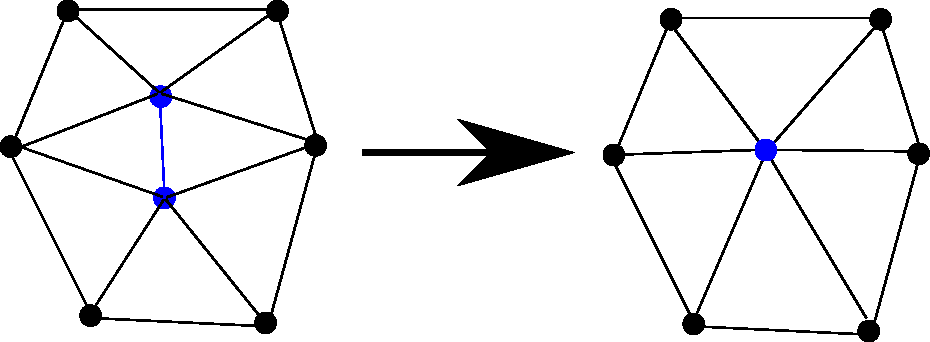
\includegraphics[width=\textwidth]{EdgeCollapse.pdf}
\end{figure}

\end{frame}


\begin{frame}{Review: Convex Shadow Casting (Stereographic Projection)}

\begin{figure}[t]
    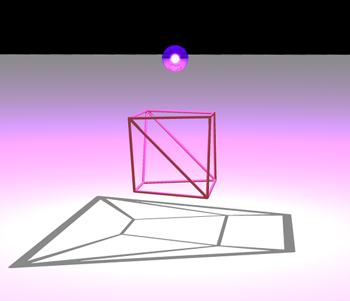
\includegraphics[width=0.7\textwidth]{shadow.png}
\end{figure}

\end{frame}


\begin{frame}{Review: Torus Euler Characteristic}

\only<1>{
\begin{figure}[t]
    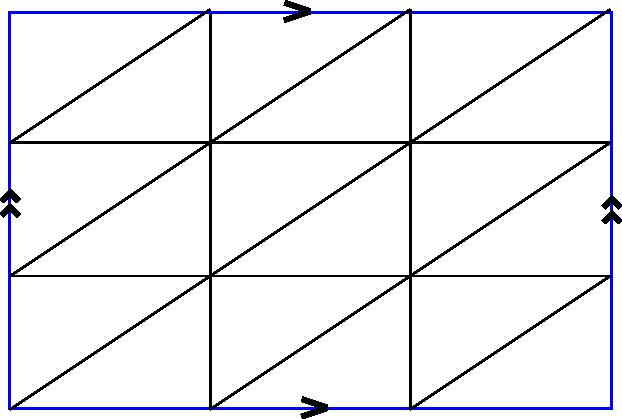
\includegraphics[width=0.7\textwidth]{FundamentalPolygon.pdf}
\end{figure}
}

\only<2>{
9 vertices, 27 edges, 18 faces: $\chi = 0$
\begin{figure}[t]
    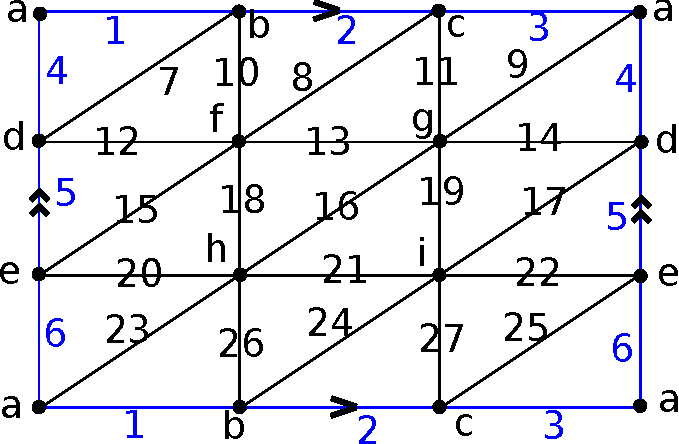
\includegraphics[width=0.7\textwidth]{FundamentalPolygonLabeled.pdf}
\end{figure}
}

\only<3>{
\begin{figure}[t]
    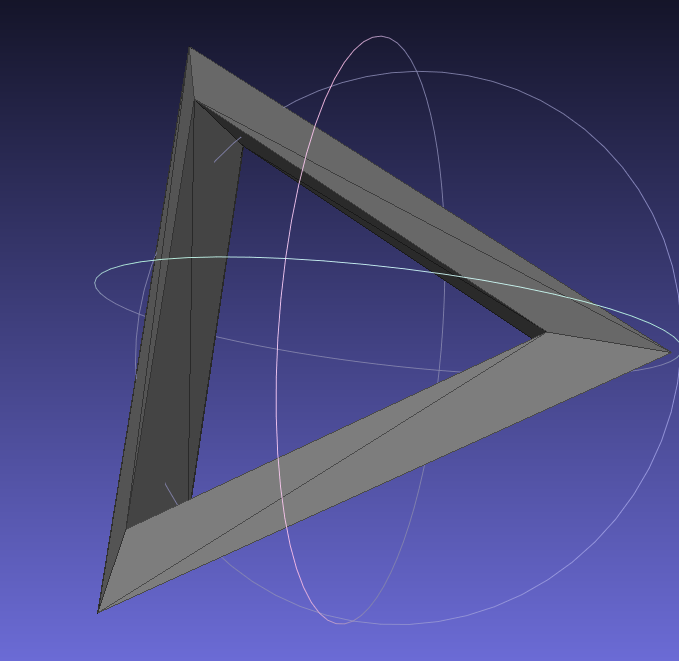
\includegraphics[width=0.7\textwidth]{3x3Torus.png}
\end{figure}
}

\end{frame}

\begin{frame}{Duplicating Spheres}

What's the euler characteristic of two spheres?

\begin{figure}[t]
    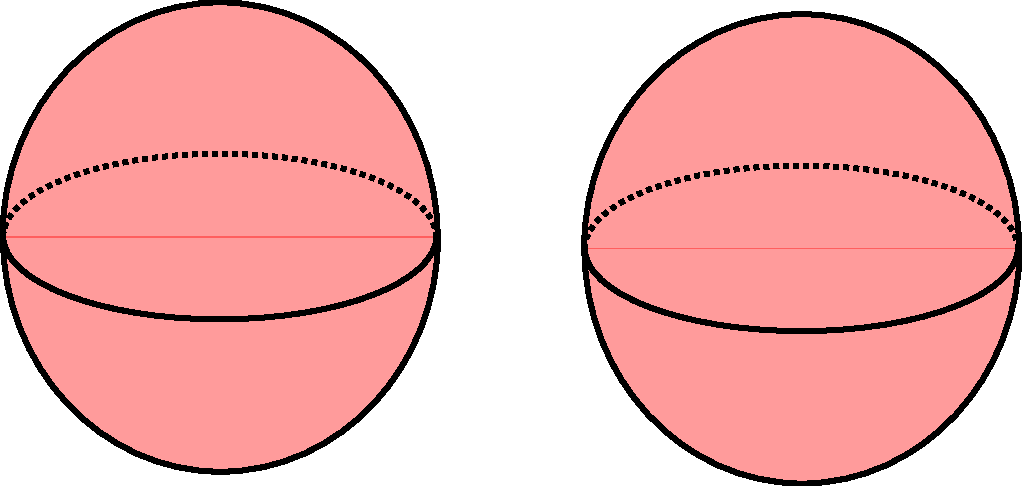
\includegraphics[width=\textwidth]{2Spheres.pdf}
\end{figure}


\end{frame}


\begin{frame}{Duplicating Tori}

What's the euler characteristic of two tori?

\begin{figure}[t]
    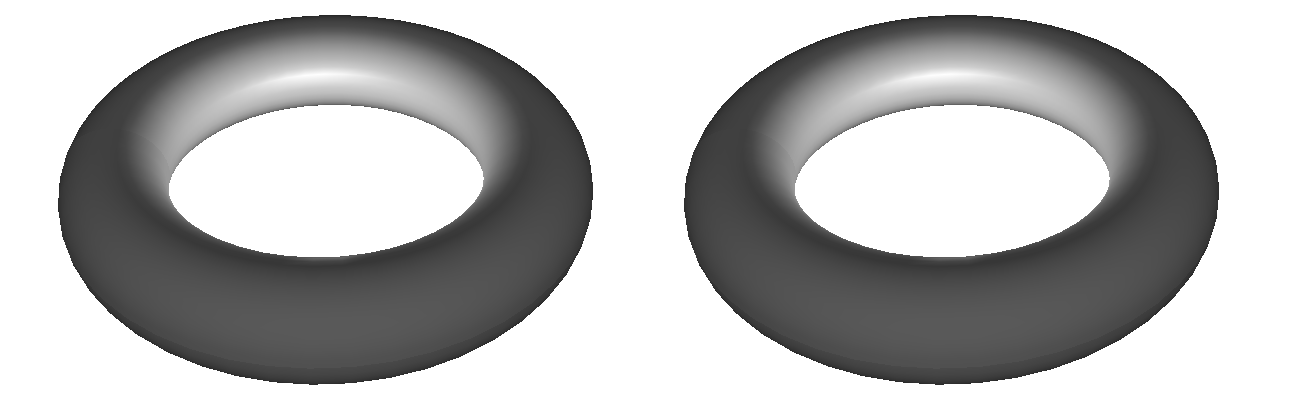
\includegraphics[width=\textwidth]{2Tori.png}
\end{figure}

\end{frame}

\begin{frame}{Connected Sum}

$T_1 \# T_1 = T_2$

\begin{figure}[t]
    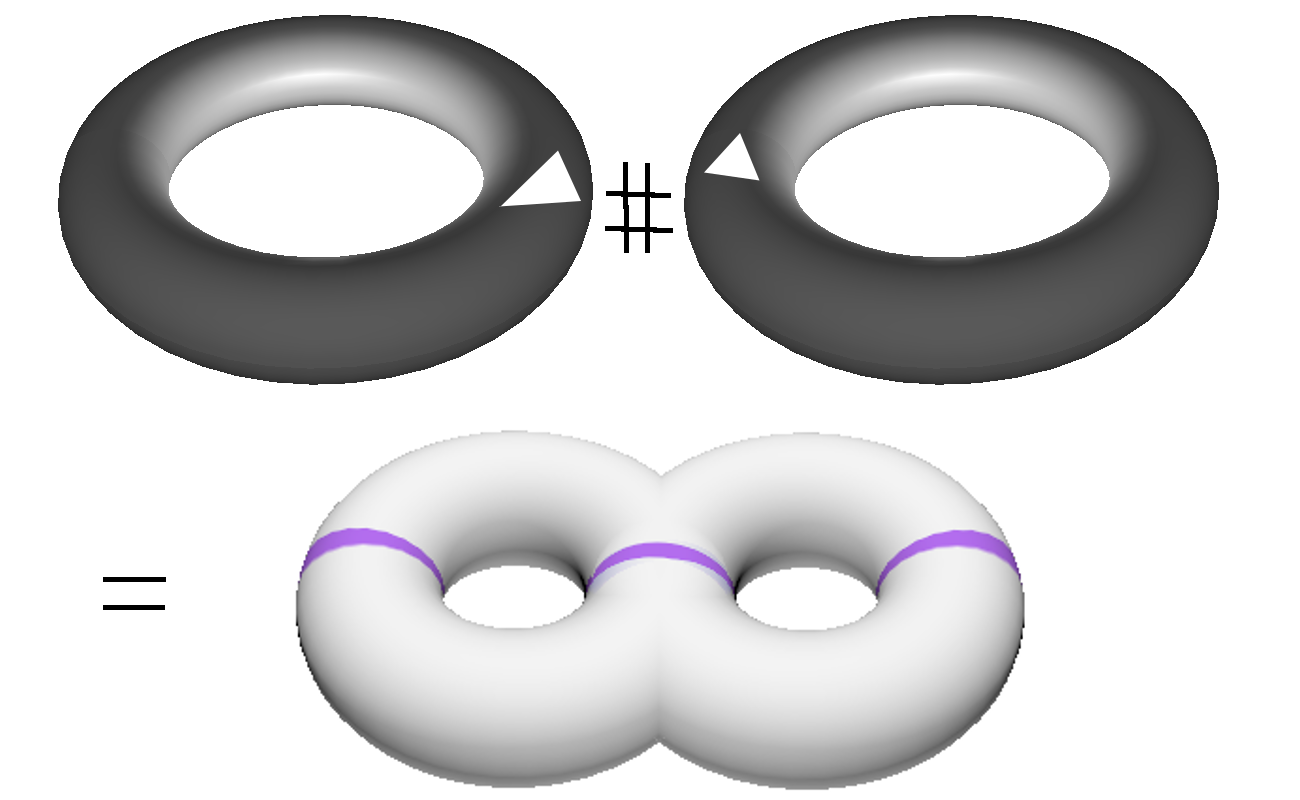
\includegraphics[width=\textwidth]{ConnectedSum.png}
\end{figure}

\end{frame}


\begin{frame}{Connected Sum}

$T_1 \# T_1 = T_2$

What is the Euler characteristic?

\begin{figure}[t]
    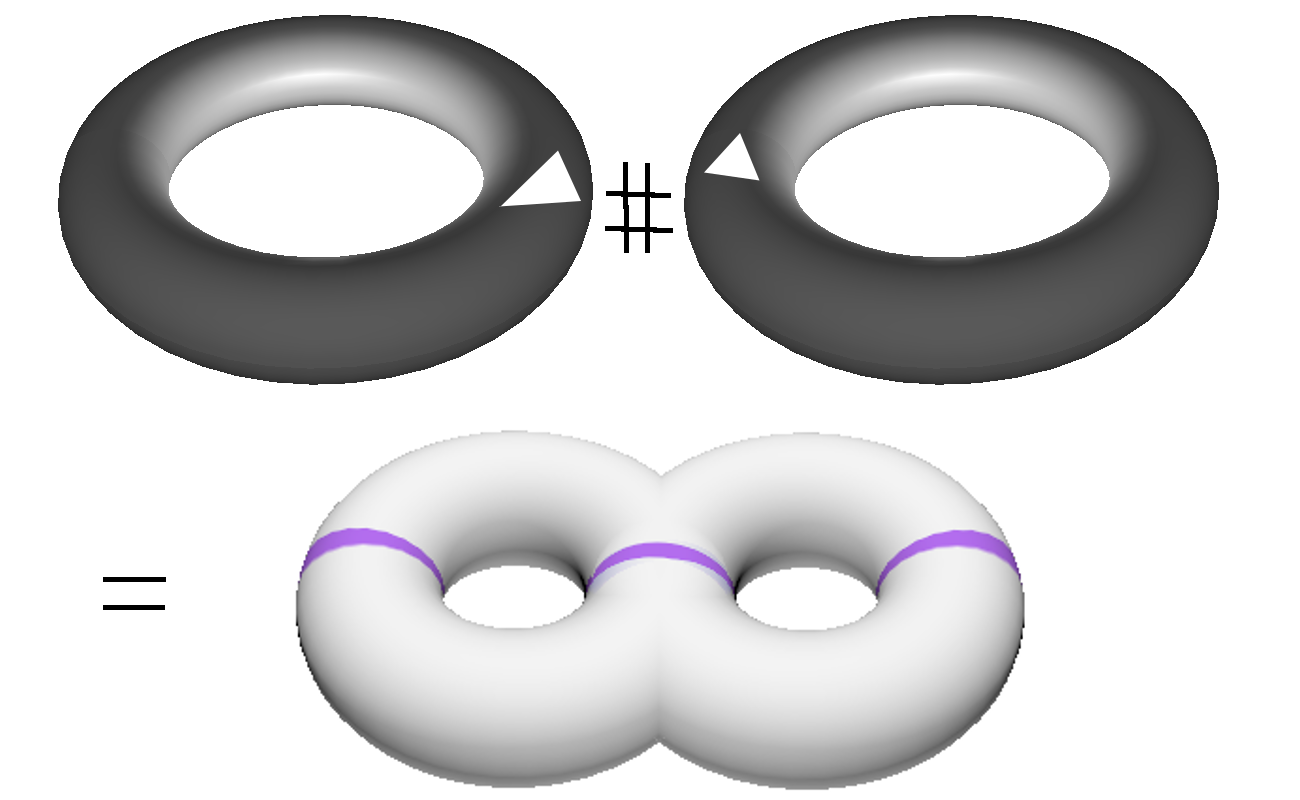
\includegraphics[width=0.6\textwidth]{ConnectedSum.png}
\end{figure}

\end{frame}


\begin{frame}{Connected Sum: g Tori}

What is the Euler characteristic of $T_N = T_1 \# T_1 \# \hdots \# T_1$ g times?

\uncover<2->{

\[ \chi = 2 - 2g \]


}

\uncover<3->{
\begin{itemize}[label=$\blacktriangleright$]

    \item $g$ is known as the ``genus''

\end{itemize}
}

\end{frame}

\begin{frame}{Connected Sum with Spheres}

What is the connected sum of a sphere with a sphere?

\end{frame}

\begin{frame}{Connected Sum with Spheres}

What is the connected sum of a torus with a sphere?

\end{frame}


\begin{frame}{Boundaries / Discs}

\only<1>{
\begin{figure}[t]
    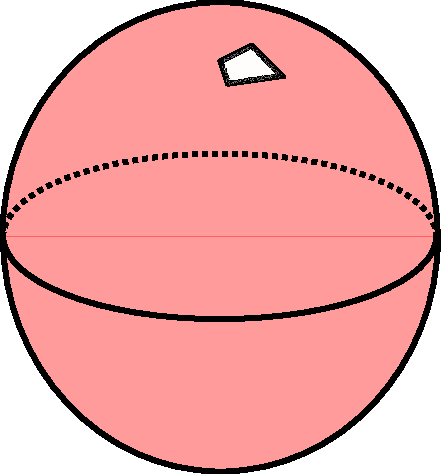
\includegraphics[width=0.45\textwidth]{SphereBoundary.pdf}
\end{figure}
}

\only<2>{
\begin{figure}[t]
    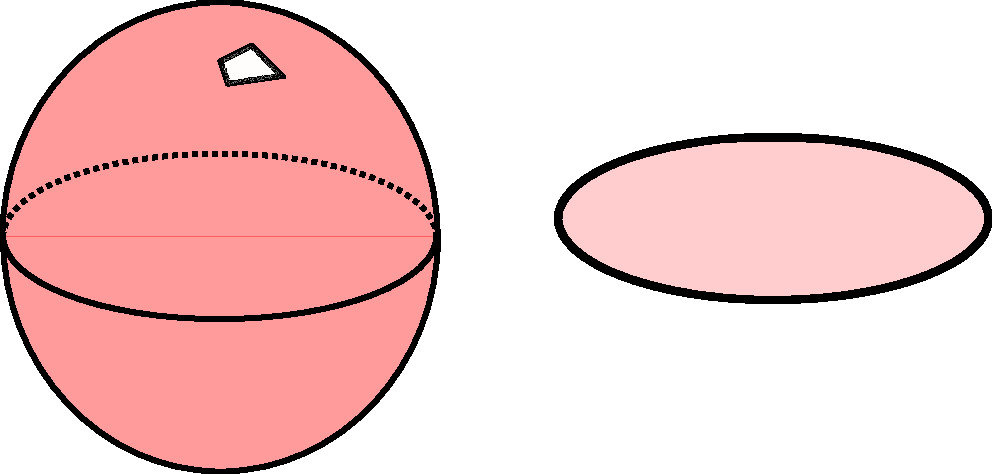
\includegraphics[width=\textwidth]{SphereBoundary_WithDisc.pdf}
\end{figure}
}

\end{frame}


\begin{frame}{Euler Characteristic: Homology}

\[ \chi = \beta_0 - \beta_1 + \beta_2 \]

\begin{itemize}[label=$\blacktriangleright$]

\item $\beta_0$: Number of connected components

\item $\beta_1$: Number of independent loops/cycles

\item $\beta_2$ Number of independent voids

\end{itemize}

\end{frame}


\begin{frame}{Something With Euler Characteristic of 3?}


\end{frame}


\begin{frame}{Table of Contents}
\begin{itemize}[label=$\vartriangleright$]
	\item Connected Sums, Genus, Boundaries
\end{itemize}

\begin{itemize}[label=$\blacktriangleright$]
	\item Mesh Data Structures
\end{itemize}
\end{frame}

\begin{frame}{Order of Edges in Planar Graph}

\[ V - E + F = 2 \]

\uncover<2->{
\begin{itemize}[label=$\vartriangleright$]
\item There are at least 3 edges per face, and each edge is on the boundary of 2 faces for a {\em manifold mesh}
\end{itemize}
}

\uncover<3->{
$3F \geq 2E \implies F \geq \frac{2}{3} E$
}

\uncover<4->{
$V - E + \frac{2}{3}E \geq 2$
}

\uncover<5->{
$E \leq 3V - 6 \implies E = O(3V), F = O(2V)$
}

\end{frame}

\begin{frame}{Vertices Per Polygon}

Put all vertex coordinates for each polygon

\begin{center}
  \begin{tabular}{ | l | c | r |}
    \hline
    $x_{11}, y_{11}, z_{11}$ & $x_{12}, y_{12}, z_{12}$ & $x_{13}, y_{13}, z_{13}$ \\ \hline
    $x_{21}, y_{21}, z_{21}$ & $x_{22}, y_{22}, z_{22}$ & $x_{23}, y_{23}, z_{23}$ \\ \hline
    $\hdots$ & $\hdots$ & $\hdots$ \\ \hline
    $\hdots$ & $\hdots$ & $\hdots$ \\ \hline
    $x_{F1}, y_{F1}, z_{F1}$ & $x_{F2}, y_{F2}, z_{F2}$ & $x_{F3}, y_{F3}, z_{F3}$ \\ \hline
  \end{tabular}
\end{center}

How many bytes per vertex, assuming 32-bit single precision floating point?
\uncover<2->{
\begin{itemize}[label=$\vartriangleright$]
\item 72 bytes/vertex
\end{itemize}
}

\end{frame}

\begin{frame}{Basic ``Off File'' Index-Based Format}

\begin{figure}[t]
    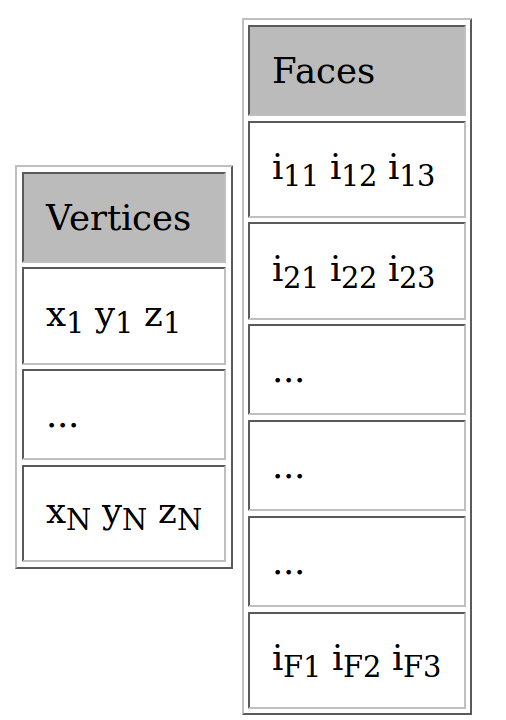
\includegraphics[width=0.4\textwidth]{OFF.png}
\end{figure}

\uncover<2->{
\begin{itemize}[label=$\vartriangleright$]
\item 36 bytes/vertex
\end{itemize}
}

\uncover<3->{
\begin{itemize}[label=$\vartriangleright$]
\item Vertex buffers, index buffers in OpenGL
\end{itemize}
}

\end{frame}

\begin{frame}{Query ``One Ring Neighbors''}

\begin{itemize}[label=$\vartriangleright$]
\item A very common operation
\end{itemize}

\begin{figure}[t]
    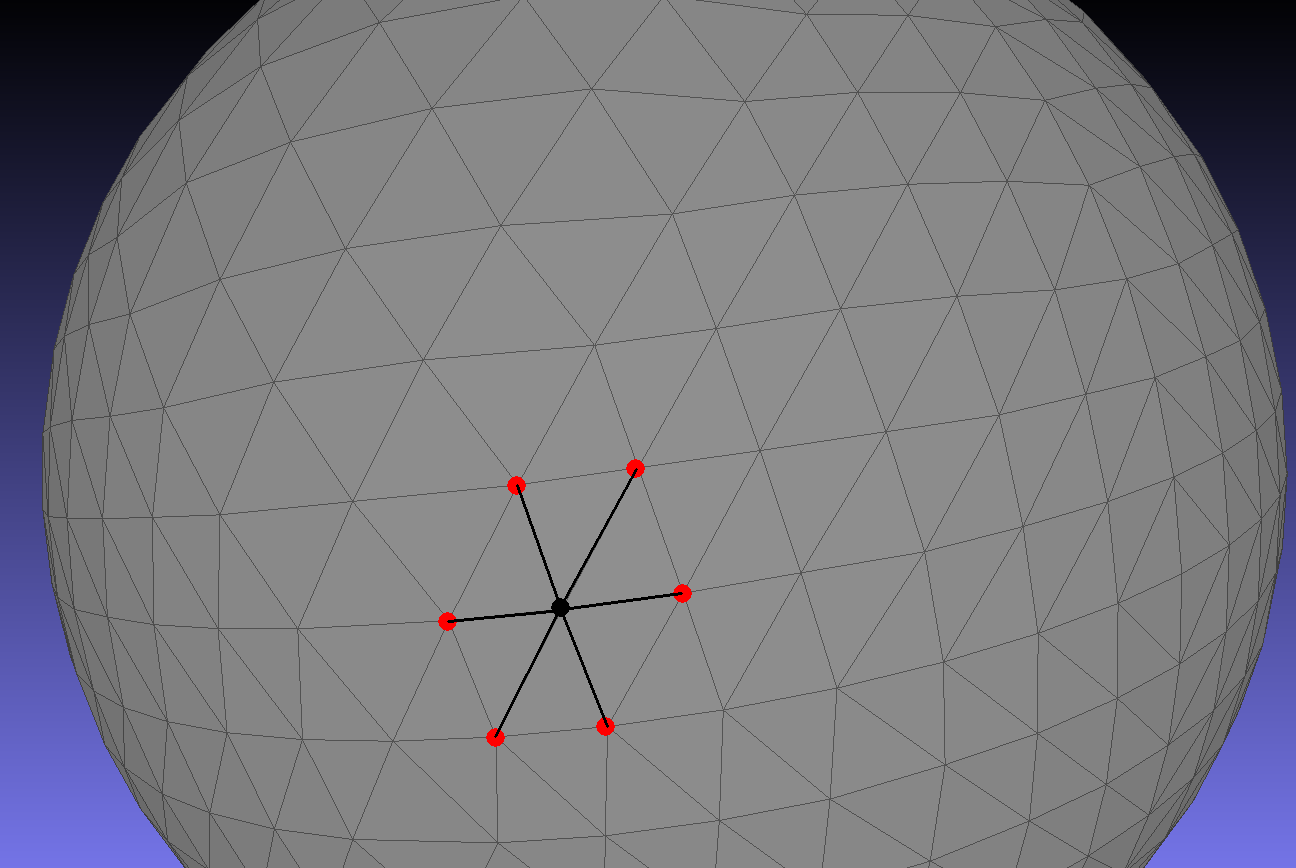
\includegraphics[width=0.8\textwidth]{Sphere1Ring.png}
\end{figure}

\uncover<2->{
\begin{itemize}[label=$\vartriangleright$]
\item Time complexity in vertex index scheme?
\end{itemize}
}

\end{frame}

\begin{frame}{Face Adjacency}

\begin{figure}[t]
    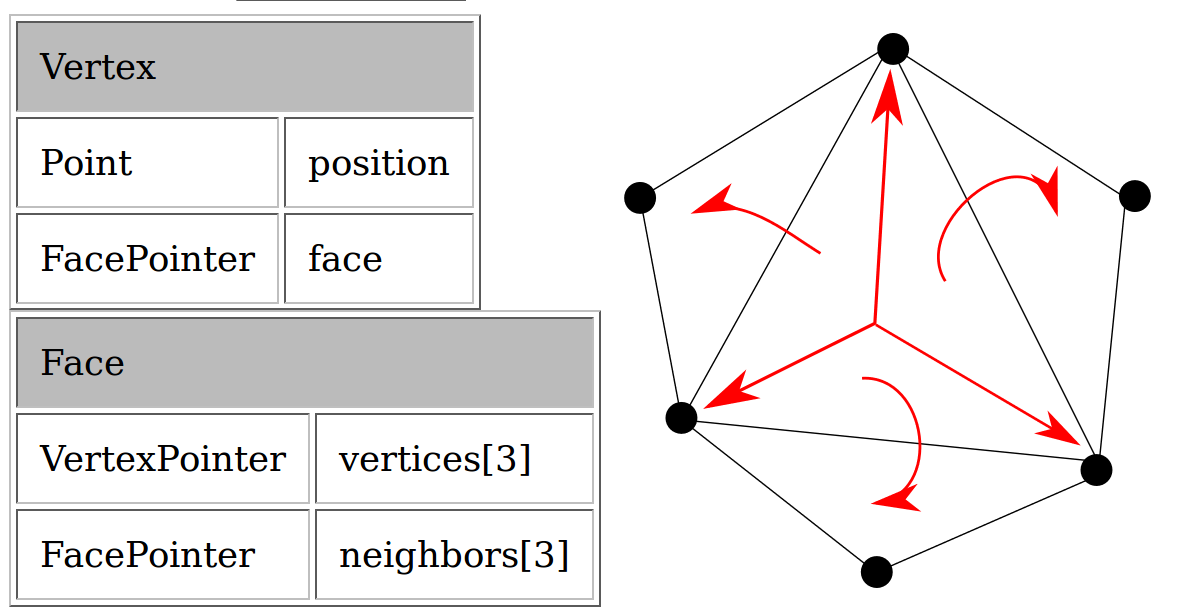
\includegraphics[width=0.9\textwidth]{FaceAdjacency.png}
\end{figure}

\uncover<2->{
\begin{itemize}[label=$\vartriangleright$]
\item 24 bytes per face, 16 bytes per vertex = 64 bytes / vertex
\end{itemize}
}

\end{frame}

\begin{frame}{GLEAT/S3DGLPY Format}

\begin{figure}[t]
    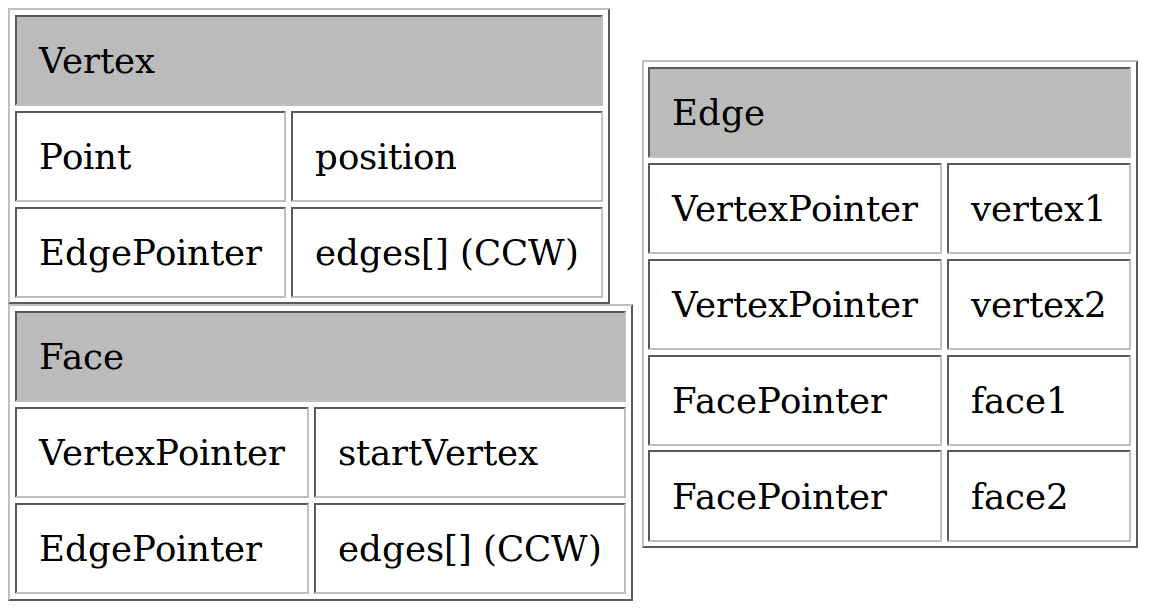
\includegraphics[width=\textwidth]{GLEAT.png}
\end{figure}

\uncover<2->{
\begin{itemize}[label=$\vartriangleright$]
\item 4*(3+6) bytes per vertex, 4*(1+3) bytes per face, 16 bytes per edge
\item $36 + 16(2) + 16(3) = 116$ bytes/vertex
\end{itemize}
}

\end{frame}


\begin{frame}{Half Edge Format}

\begin{figure}[t]
    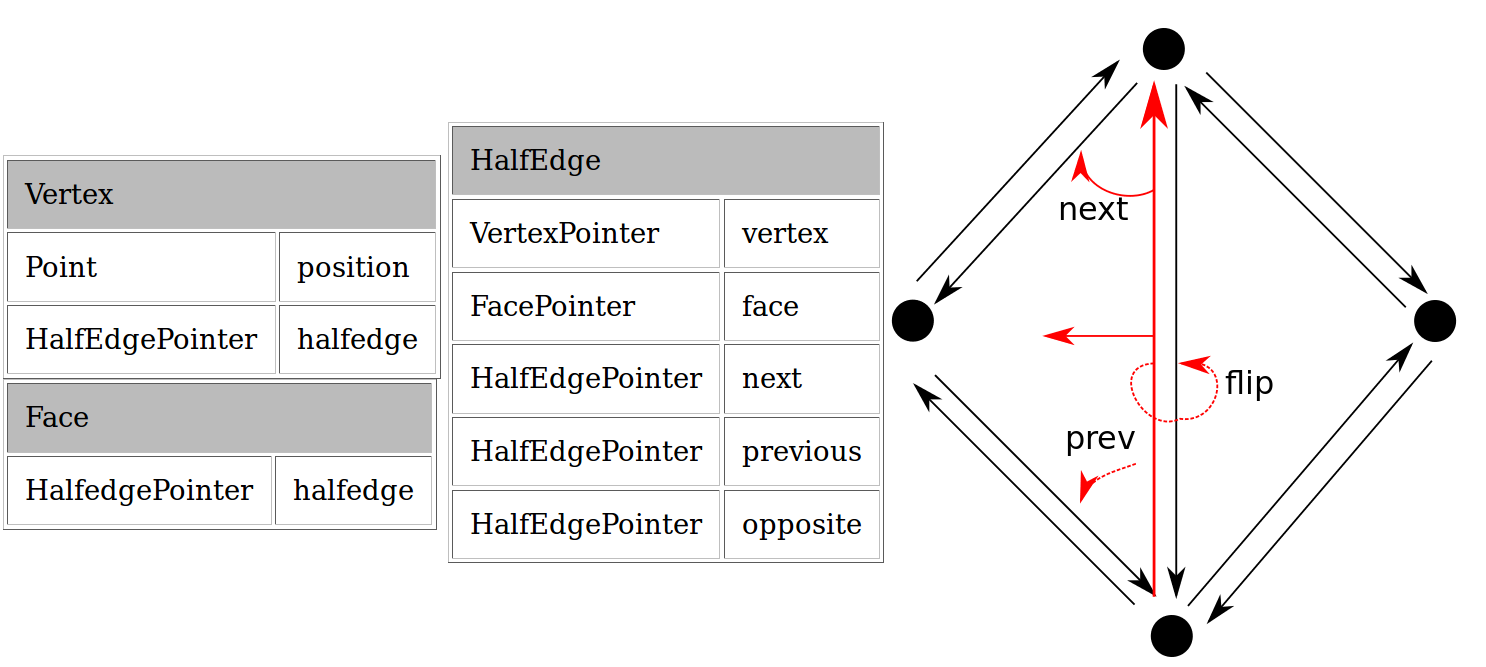
\includegraphics[width=\textwidth]{HalfEdgeIllustration.png}
\end{figure}

\uncover<2->{
\begin{itemize}[label=$\vartriangleright$]
\item 16 bytes per vertex, 4 bytes per face, 20 bytes per half-edge
\item 16 + 4(2) + 20(3)(2 halfedges) = 76 bytes / vertex = 144 bytes/vertex
\end{itemize}
}

\end{frame}

\begin{frame}{Half Edge One-Ring Neighbor}

\begin{figure}[t]
    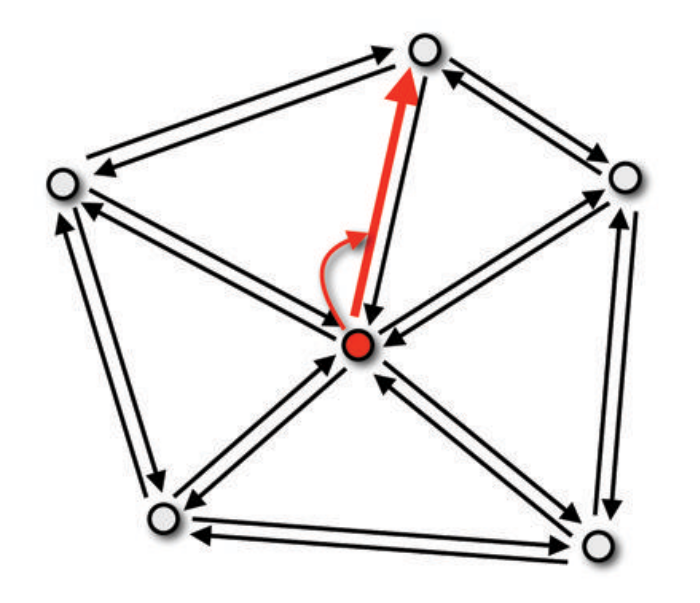
\includegraphics[width=0.7\textwidth]{HalfEdgeOneRing.png}
\end{figure}

\end{frame}

\end{document}

